\subsection{Foundations of Image Classification and Deep Learning}
%%%%%%%%%%%%%%%%%%%%%%%%%%%%%%%%%%%%%
\subsubsection{Image Classification}
Image Classification is a categorization and labeling process by mapping high dimensional pixels data to a pre-defined set of discrete classes. For decades, researchers have developed advanced classification models due to the increasing complexity in image analysis, making it critical to improve classification accuracy and reduce labor force. CNN (Convolutional Neural networks) -based approaches have significantly advanced in the field of computer vision, especially in image classification tasks, their hierarchical feature extraction mechanism, and spatially invariant filters to efficiently learn robust features of an input image.  The evolution of CNN architectures has marked a significant shift from shallow architectures to deep networks due to the evaluation of increasing complexity of datasets. In early breakthrough, AlexNet is a foundational architecture that utilises GPU(Graphical Processing Unit), and significantly improved the architecture of previous convolutional neural networks using multiple layers , dropout , ReLU activation function which mitigates the vanishing gradient problem, and data augmentation to prevent overfitting. Subsequently in GoogleNet, the inception module offers a method to introduce parallel convolutional layers with varying filter sizes, which allows the network to capture features with different scales while maintaining computational efficiency .(Noor \& Ige, 2024)  .VGGNet , on the other hand, focus on the principle of using  convolutional layers with small 3X3 filters , demonstrating that increasing the network depth could improve feature extraction capabilities. In contrast to VGGNet’s emphasis on depth , in 2015 at the ILSVRC (Image Net Large Scale Visual Recognition Challenge) , ResNet was introduced with residual connections, allowing deeper networks to be trained effectively by creating skip connections allows the features learned in the previous layers to be directly reused in the upcoming layers that facilitate the backpropagation. Recent advancements in CNN Architecture the vanishing gradient problem, diminishing feature reuse while elevate the classification error by improving the feature learning . DenseNet was introduced in 2016, follows the same methodology as ResNet,utilizing residual connections between layers . However, DenseNet establishes a dense block where it consists multiple convolution functions followed by batch normalization, ReLU activation function ,and 3x3 convolution  ,maximizes the information flow ,feature reuse and preserves the feedforward nature of the network. \cite{mohdnoor2025survey}. ResNeXt addresses the issue of diminishing feature reuse by capturing more efficient and diverse features . While traditional networks improve performance by increasing the depth, often at the cost of computational efficiency, ResNeXt introduces a third dimension : Cardinality. By integrating residual connections of ResNet with the parallel path methodology of Inception modules, ResNeXt manages complex interactions without a computational explosion.

pre-trained cnn models with ImageNet dataset:
\begin{figure}
    \centering
    \includegraphics[width=0.5\linewidth]{/Users/zeynepoykuerdem/master_thesis/figures/fig_cnn_top_five_errors_imagenet.png}
    \caption{The classification error comparison between pre-trained models with ImageNet dataset}
    \label{fig:pre-trained cnn models}
\end{figure}
\cite{mohdnoor2025survey}
%%cnn architectures evolution in performance,imagenet datasetinden bahset

Collectively, these innovations illustrate clear evolutionary progression in CNN design, each share common underlying principles that govern how convolutional neural networks function with visual information. Understanding these fundamental concepts is essential for further analysis on memorization phenomenon in CNN architectures.
%%%%%%%%%%%%%%%%%%%%%%%%%%%%%%%%%%%%%
\subsubsection{Brief Overview of CNN(Convolutional Neural Network) Components}
The Convolutional Neural Network is a feedforward neural network designed to automatically extract hierarchical features from input data with convolutional structures .Unlike traditional feature extraction methods, CNN does not require manual feature engineering, as learning complex features hierarchically. 

A key characteristic of CNNs is their hierarchical learning mechanism. Early convolutional layers capture low-level visual patterns such as edges, corners, and textures, while deeper layers can progressively integrate this low-level information into more complex, abstract representations, including object parts and semantic concepts. This hierarchical learning enables CNNs to achieve remarkable performance in various computer vision tasks, including image classification, object detection, and semantic segmentation [13] \cite{fel2025sparksexplainabilityrecentadvancements}. Additionally, the specialized structure of CNN, which includes convolutional layers, pooling layers, and fully connected layers, facilitates parameter sharing and reduces the total number of learnable parameters, making them efficient for processing high-dimensional image data [14]\cite{Bilal_2018}, [15]\cite{Nia23}. 

The transition from traditional structure to modern structural innovations has empowered CNNs with higher dimensional capacity. While these advancements, such as non-linear activations , residual learning , more layered structure, enable the model to capture intricate details. 

Despite the elevated structure, and high classification accuracy, the inherent opaqueness of these complex models often limits their interpretability, making it challenging to understand the underlying reasons for their predictions [16]\cite{10.1145/3563691}. This lack of transparency becomes particularly critical in image classification tasks, where high accuracy may mask memorization effects.  

Consequently, understanding of CNNs encode and utilize learned features requires the use of explainable artificial intelligence (XAI) techniques, which aim to reveal and interpret the internal representations and decision making mechanisms of deep neural networks.

%%%%%%%%%%%%%%%%%%%%%%%%%%%%%%%%%%%%%
\subsubsection{ Feature Extraction vs. Classification}

The architecture of a Convolutional Neural Network is primarily characterized by two stages : feature extraction and classification. Understanding the distinction between these two stages is crucial for evaluating the reason behind the irrelevant pixel-level artifacts identified in image classification tasks.

\textbf{The Role of Feature Extraction}


\begin{theorem}
\label{Convolutional Operation}
The convolution of an input x with a filter w, parameterized by Q = {w,b}, for a single channel, is defined as:
    \((x\otimes w)_{i,j}=\sum_{m}\sum_{n}x_{m,n}.w_{i-m,j-n}+b\)
where \(\otimes\)  denotes the convolution operation. For multichannel inputs, this operation is performed independently for each channel and summed to produce a single output.
\end{theorem}



The feature extraction stage, comprising convolutional and pooling layers, performs a hierarchical decomposition of a raw data input into more abstract and semantically meaningful representations. Convolutional layers, by applying filters to the input image, generate a feature map . This feature map highlights the specific patterns and features, such as edges, corners , and textures, present in the image [16]\cite{Fauzan2021PleuralEC}. Subsequently, pooling layers facilitates the reduction of dimensionality through down sampling. This reduction helps to reduce complexity by retaining the most salient features, while also enhancing the model's robustness to spatial variations and minor distortions in the input [13]\cite{fel2025sparksexplainabilityrecentadvancements}. 

\textbf{The Role of Classification}

Following the feature extraction stage, fully connected layers also known as multilayer perceptrons take the flattened output of the feature extraction to perform a global synthesis of the learned patterns. Each neuron in these layers is connected to every activation in the previous layer, performing a linear transformation followed by a non-linear activation function. 

Mathematically, this operation is expressed as :

\begin{theorem}
\label{The Multilayer Perceptions (MLP)}
    \(y\_{i}=\sigma(Wx+b)\)
 where x denotes the input vector, W denotes the weight matrix, b is the bias term, and \(\sigma\) is the non-linear activation function.   
    
\end{theorem}

This process functions as a decision-maker, integrating high dimensional feature vectors into specific semantic labels to produce the final classification. While convolutional layers focus on local spatial hierarchies, the fully connected layers interpret these features globally to determine the final probability distribution of the classes.

%%%%%%%%%%%%%%%%%%%%%%%%%%%%%%%%%%%%%
\subsection{The  Taxonomy of Explainable AI in Image Classification}
This section establishes a comprehensive  taxonomy of Explainable Artificial Intelligence and delves into mathematical foundations . The explorations focus on the categorization of XAI methods ante-hoc versus post-hoc, global versus local, and model-specific versus model-agnostic techniques, while integrating the underlying mathematical principles that govern their interpretability \cite{ferry2023interpretability,10.1145/3709367,Schwalbe_2023}. The essential focus is directed towards post-hoc techniques, given their substantial used in giving explanations in complex, black-box models. Understanding the post-hoc techniques ,generally fall into Attribution Methods and  Model-Agnostic Local Explanations, leverage the understanding of the phenomenon of Memorization .

Following flowchart illustrates the taxonomy of explainable ai in this thesis.
\newpage
\begin{figure}
    \centering
    \includegraphics[width=0.5\linewidth]{/Users/zeynepoykuerdem/master_thesis/figures/Flowchart.jpg}
    \caption{The flowchart of taxonomy explanation}
    \label{fig:xai-taxonomy} 
\end{figure}



\subsubsection{The Categorization by Stage }
\begin{figure}
    \centering
    \includegraphics[width=0.5\linewidth]{/Users/zeynepoykuerdem/master_thesis/figures/stage.png}
    \caption{Different Interpretability Approach in Deep Learning Model}
    \label{fig:stage-categporization}
    
\end{figure}

XAI methods can also  be described based on the stage of interpretability. This categorisation is derived at which the explanation is generated: during the model design ( ante-hoc) or after the model has been trained (post-hoc). 

\paragraph{Ante-hoc Interpretability}

Ante-hoc Interpretability are known as intrinsic explainability, transparent or glass-box models, which are inherently interpretable because of their uncomplicated structure.(Retzlaff et al., 2024) This simpler structure allows direct comprehension of internal decision making process . Despite their intrinsic interpretability of ante-hoc approaches, the predictive power of such models often diminishes with increasing complexity of the underlying features and data, specifically in high dimensional image processing tasks, where the straightforward linear relationships and decision trees struggle to capture complex patterns in image pixel regions. 

\paragraph{Post-hoc Interpretability}

Contradictory to ante-hoc methods, post-hoc interpretability refers to the techniques which analyse and interpret the decision-making process of a trained model after it has made predictions, providing explanations how the model arrived at its outputs. This approach focuses on the need to simplify the decision logic of black-box models to human friendly forms.

In high-dimensional domains such as image classification, achieving high level of prediction performance is often prioritized over transparency. Additionally, the unknown relationships and intricate patterns that constrained in simpler models necessitate the use of post-hoc approaches that can reveal the hidden complexities. For this reason, post-hoc methods are indispensable for trustworthy deployment of deep learning systems.

Post-hoc techniques are commonly divided into two important categories : Model Agnostic, and Model Specific methods.
\clearpage
\subsubsection{The Categorization by Scope }

Scope un anlami

The categorisation on the basis of Scope mainly involves in two directions: global explanations, and local explanations.

\paragraph{Global Explainability}


Global Explainability aims to provide global understanding of a model’s overall logic, revealing the general relationships between features and the model’s predictions overall the entire dataset (Agrawal \& Sharma, 2024). An explanation is considered as global if the explanator othen than why of local explanations, provides also how a decision is made.(Schwalbe \& Finzel, 2021)

(Feature Importance, Partial Dependence Plots, and Surrogate Models are common techniques employed for global interpretability, offering insights into the average behavior of a model across its entire input space (Černevičienė \& Kabašinskas, 2024; Höhl et al., 2024). This approach allows for comprehension of the model's general tendencies and the influence of features on its global output (Khan et al., 2024). )
\paragraph{Local Explainability }

Conversely, Local Explainability focuses on the reasoning behind a specific prediction for a single data instance, addressing how individual features contribute to the prediction for a particular input. This distinction is crucial for tailoring XAI methods to specific user needs and tasks. Specifically  in image classification tasks, understanding why a model classifies a particular image , requires localised explanations that highlight specific regions or features within that individual image contributes to the decision . 
\clearpage

\subsubsection{Local Post-hoc Interpretation Techniques }

\paragraph{Model-agnostic techniques }

Regardless of the architecture of the model, these methods aim to explain the decision making process of the model flexible and applicable across diverse machine learning models.(Devireddy, 2025; Ramachandram et al., 2025)This independence enables a universal framework, by simultaneously analysing the inputs and outputs without gaining model insights such as weights or parameters. However, such methods typically approximate the model locally or globally, which may limit their faithfulness.

\subparagraph{Perturbation-based methods }
Perturbation-based methods operate by systematically perturbing parts of the input image and observing the corresponding changes of perturbed parts in the model’s predictions.This approach is model-agnostic, as it does not rely on the internal architecture of the model, and can therefore be applied across wide range of models . As they rely on observing changes in the model’s output in response to input perturbations, can be performed in black-box settings. Since the information in images is typically highly correlated across neighbouring pixels, perturbing individual pixels  is unlikely to influence on the prediction.(Pihlgren \& Främling, 2024). Instead, the input image is commonly perturbed at the level of segmented regions.Each segmented regions is then sampled with respect on the predefined sampling strategy that determines which regions should be perturbed or occluded. Based on this strategy, multiple perturbed instances are generated , while the remaining regions are kept unchanged. Each perturbed segment  is then passed through the trained model, and resulting in a measure of the prediction change with respect to the original output. Based on these prediction differences, an attribution score is assigned to each region, reflecting its relative importance in the model’s prediction alterations. Finally, these scores are aggregated to generate a saliency map, a visual explanation that  highlights influential regions of the image.

Representative perturbation-based methods include LIME, Kernel SHAP which all utilize perturbation by leveraging individual features in a model.


\paragraph{Model specific techniques}

Conversely, model specific techniques leverage the internal structure of the AI model or algorithm, to provide more insightful and effective explanations such as learned parameters or gradients . These methods often tailored to specific machine learning models, especially deep learning models. While this model-specific explanation techniques can yield more precise and architecture dependent explanations , their applicability into practice if often limited, this incapability restricts their acceptance into mainstream research of XAI methods.(Hassija et al., 2023). Additionally, this approach is inherently applicable in Convolutional Neural Networks, where convolutional layers , feature maps, and gradients are directly utilise to highlight specific regions of the input image contribute most to a prediction.

\subparagraph{Gradient-based methods}
Gradient-based methods, are widely used in convolutional neural networks, assume that the parameters of the model are accessible.These techniques employ forward and backward pass to estimate the  influence of each input pixel respect with the original output. During the  forward-pass ,the input image is passed through a deep neural network to generate a prediction score for a specific class. In the subsequent backward step, instead of adjusting weights , the gradient of the output score using back-propagation with respect to the input pixels is computed. This gradient then indicates the sensitivity of prediction to slight changes in each pixel, thereby highlighting which features the model is important related to model’s prediction.

Saliency Maps, Grad-Cam, and Integrated Gradients are commonly used techniques under the gradient-based methods .
\subparagraph{Decomposition-based methods}
Decomposition-based techniques decompose the model output layer by layer into different features and showing the contribution of each input feature relevance towards the final prediction. While  gradient-based approaches that measure  the sensitivity of the output to small changes in input features, decomposition-methods focus on highly localised features which results in more precise attributions.

A prominent example is Layer-wise Relevance Propagation (LRP), which systematically redistributes the prediction score to the previous layer , based on specific LRP rules to assign a relevance score to each input feature.
\clearpage

\clearpage
%%%%%%%%%%%%%%%%%%%%%%%%%%%%%%%%%%%%%
\subsection{The Phenomenon of Memorization}
%%%%%%%%%%%%%%%%%%%%%%%%%%%%%%%%%%%%%
%%%%%%%%%%%%%%%%%%%%%%%%%%%%%%%%%%%%%
Memorization is a phenomenon where machine learning models, particularly deep neural networks, retain information about specific training examples instead of learning patterns that generalize well to unseen data.This concept is crucial in understanding the behaviour of the model, especially in the context of overfitting, where a model achieves high accuracy   on training data but performs poorly on the test set. The high capacity and complex parameter space of deep neural networks enable these models to store detailed information from individual training samples, which causes poor generalisation and makes them susceptible to capturing noise rather than robust, transferable features \cite{ali_raza_537a9747}. 

Researchers have further refined the concept of memorisation,  often distinguishing mainly between Memorization Learning , which refers to the process of learning specific details or particular features of examples, and Pattern Learning which focuses in on extracting common patterns or generalised features  in the data \cite{jiaheng_wei_8cfd95ec}. Understanding the distinction is crucial for diagnosing model’s behaviour, and developing explanaible AI systems that can reveal whether a  model’ decision is driven by the memorisation or meaningful, generalisable patterns. 

The following subsections expand on these ideas: Conceptual Deepening,  provides the theoretical and mathematical background of Memorization giving ; Generalisation Tradeoff which examines the distinction between Generalisation vs. Memorisation;Memorisation in Convolutional Neural Networks  examines the reason why CNNs are particularly prone to memorisation; and  Mitigation Techniques for Memorization survey the methods to reduce memorization in deep learning models.
%%%%%%%%%%%%%%%%%%%%%%%%%%%%%%%%%%%%%
\subsubsection{Conceptual Deepening of Memorization}
Memorization refers to the ability of model’s parameters to store and recall specific training examples rather than learning underlying data distributions. The traditional view of generalization posits that deep neural networks due to their over-parameterized, complex structure results in overfitting the training set yields poor generalization to validation set and test sets \cite{ian_goodfellow_5e6a80c8}. However , empirical evidence shows that deep neural networks often achieve excellent generalisation performance , ‘well’ accuracy score with sufficient capacity \cite{devansh_arpit_9e68508c}. \cite{chiyuan_zhang_bd8f0549} highlight a remarkable property of deep neural networks: despite achieving zero training error, implies overfitting, these models can still maintain low test error. The real question is how these models achieves this state-of-art conditions? \cite{chiyuan_zhang_bd8f0549}furthers this question by varying experimental conditions on neural networks ,examining how generalization performance changes under data corruptions and label corruptions on CIFAR-10.  Importantly ,even when the corruption destroys the relationship between images and labels, networks learning capability slows down yet neural networks are still able to fit  the training data perfectly. 
- Burda generalization error formulayi ver
Furthermore, this experiment highlights the rising testing error under the data corruption, emphasizing that there is a strong memorization capability. These oservations could not able to explain with a statistical learning theory where we imply different complexity measures, controlling generalisation error. These include VC Dimension \cite{vladimir_vapnik_d1c1a1dc}, which quantifies the complexity of a hypothesis space independently of the underlying data distribution; and its pseudo-dimension. Rademacher complexity \cite{shai_shalev_shwartz_c0318cbc}, refines VC Dimension including distribution dependent complexity that naturally apply to real-valued  and multi-class function classes. Finally, Uniform stability measures the sensitivity of a learning algorithm to small perturbations in the training set.
The observed distinction between generalization and memorization underscores that achieving low training error do not necessarily imply that meaningful patterns have been learned. Classical complexity measures alone appear insufficient to fully explain this paradox. To explain memorization beyond classical complexity measures, it is essential to examine the nature of the information being retained. Specifically, recent literature distinguishes between two fundamental mechanisms: label memorization and feature memorization. 
\paragraph{Label versus Feature Memorization}
Label Memorization refers to the phenomenon where models memorize the labels in training datasets without learning the relevant patterns that the label can be predicted . This propensity for label memorization, cannot be explained by the classical generalization formula , which is the sum of the empirical error in training set and the generalization gap controlled by the model complexity parameter and the empirical error.  \cite{chiyuan_zhang_bd8f0549}, conducted experiments demonstrating the label memorization phenomenon on CIFAR-10. Their results show that, models trained on datasets with random labels achieve almost  zero-training error, while experiencing severe generalization degradation. Specifically, they observed that as label corruption increases 0\% to 100\%, the convergence increases significantly, yet models continue to memorize the corrupted labels, resulting in high  generalization error (since the training error is 0). 
In contrast, feature memorization involves the model learning and retaining spurious features that are uncorrelated with the true underlying data distribution.\cite{simone_bombari_23e6de9b} \cite{yang_yu_4720d432} This type of memorization, stated in (Yu et al., 2023) , is separable based on the model’s output early in training. In the experiment, a colored MNSIT used as an example of spurious correlations. Each digit in MNSIT datasets is a class , where the majority of digits have a particular color, and the remaining digits are in other colors. The model, therefore, learn to associate the color with the core feature instead of the digit’s shape, leading to poor generalization on correlations where the spurious correlation between color and digit is broken \cite{chenyu_you_e79f4b0f}.  While feature memorization describes the model’s propensity for learning uncorrelated patters, a closely related phenomenon known as Shortcut Learning explains the mechanism behind this behaviour.
\paragraph{Shortcut Learning and its Implications}
Shortcut Learning in neural networks, occurs when a model achieves high performance on a standard benchmark, not by comprehending the underlying data correlations between input and output, but using shortcut features or exploiting trivial associations that fail in generalization performance \cite{robert_geirhos_e33ec72d}.  As an example , a model trained to distinguish between wolves and huskies might learn to associate snow in the background with wolves, rather than focusing on the animals' distinct facial features \cite{chenyu_you_e79f4b0f}. Another example is provided in (Geirhos et al., 2020) an image classification task where the model is trained to identify stars and moons , instead of learning the actual shape of the  objects , it exploit the location of the images .This indicates that the model has learned a “shortcut”- a decision rule that performs well on training distribution but fails in generalization tests. 

This phenomenon has serious implications in applications requiring robustness and fairness . In the article \cite{joy_buolamwini_0378cfd5} conducted an experiment over the 3 different parliamentary benchmarks  to illustrate the social amplification on neural networks. Given benchmarks were IJB-A US Government Benchmark published by NIST ( National Institute of Standards and Technology) in 2015 and Adience is a widely-used face image dataset originally developed for gender and age classification; yet these models overrepresented lighter males, underrepresented darker females, thereby underrepresented of darker individuals in general. PPB ( Pilot Parliaments Benchmark) was therefore focused on achieving better intersectional representation  in balanced datasets. To provide a comprehensive evaluation of these biases in real world applications; examined three commercial gender classification systems: Microsoft, IBM, and Face++. These classifiers were selected because they represented the state-of-the-art in facial analysis technology and were widely deployed in commercial products during that period of time. The result demonstrates that even with a balanced representation of protected characteristics, models may still exhibit bias amplification in darker-skinned people. Especially the highest error rates  were observed for darker-skinned females ranging from 23.8\% for Microsoft to 36.0\% for Face++ and 33.1\% for IBM \cite{anoop_krishnan_6fbfbe57}. The underlying cause is that the models tend to learn the shortcut way ,  relying on “facial geometries” and “gender norms“ specific to the majority group of population in the training set, failing to generalize to minority subgroups.

When a model’s decision boundary is defined by memorized shortcuts rather than learning robust semantic representations, it becomes vulnerable to critical security issues. In the following section , memorization based fragility is targeted through white-box adversarial attacks, specifically focusing on the mechanisms of FGSM and PGD.
\begin{table}
    \centering
    \begin{tabularx}{\textwidth}{|X|X|X|X|X|X|X|X|X|X|}
    \toprule
    \multicolumn{10}{|c|}{\textbf{Dataset Properties Comparison between Benchmarks}} \\
    \midrule{}
    \textbf{Dataset} & \textbf{n} & \textbf{Female} & \textbf{Male} & \textbf{Darker} & \textbf{Lighter} & \textbf{DF} & \textbf{DM} & \textbf{LF} & \textbf{LM} \\
    \midrule{}
 PPB   & 1270  & 44.6\% & 55.4\% & 46.4\% &53.6\% & 21.3\% & 25.0\% & 23.3\% & 30.3 \%\\
 IJB-A & 500  & 24.6\% & 75.4\% & 20.4\% & 79.6\% & 4.4\% & 16.0\% & 20.2 \% & 59.4 \%\\
 Adience & 2284 & 52.0\% & 48.0\% & 13.8\% & 86.2\% & 7.4\% & 6.4\% & 44.6\% & 41.6 \% \\

 \bottomrule
\end{tabularx}



\end{table}
%%%%%%%%%%%%%%%%%%%%%%%%%%%%%%%%%%%%%
\subsubsection{White-Box Attacks in DNN and Its Correlation with Memorization }
To evaluate the security implications of memorization, this section focuses on White-Box attacks. Unlike Black-Box scenarios where the attackers could not have any knowledge of the internal architecture, parameters or training data of the model, White-Box scenarios allows studying memorization by examining model’s vulnerabilities, specifically “jagged” points where the model can be systematically exploited. To understand these vulnerabilities, the adversarial space should be defined. Adversarial Space according to \cite{chio_clarence_9b691fc0}, is a result of imperfect representation in training data where the entire input space cannot be provided . This imperfect representation of the input space provided in training data in white-box models , allows Attackers exploiting “Sensitivity” of memorized features  and moving the direction that the model is “weakest”. In standard training , gradient-descent is utilized as an  optimization algorithm to minimize the cost function by updating model weights , attackers used the transparency of white-box models to reverse this logic. Instead of updating weights to minimize loss, they keep the weights fixed and perturb the input pixels to maximize the loss function. To illustrate this phenomenon , we will examine two primary gradient-based strategies: Fast Gradient Sign Method( FGSM) and Projected Gradient Descent (PGD).
\paragraph{Fast Gradient Sign Method (FGSM)}
The Fast Gradient Sign Method (FGSM) , introduced in  \cite{ian_goodfellow_5e6a80c8} adding subtle perturbations into the gradient of the cost function with respect to the original input to maximize the misclassification and thereby highlighting vulnerabilities in deep learning networks. Specifically, the sign of the gradient indicates the direction in which the input pixels must be altered to increase the loss function J. By moving the input in this direction by a small step ϵ, FGSM creates an adversarial image xadv that is often indistinguishable from the original image without visible changes but results in incorrect classification by the model.  A key theoretical insight behind FGSM, is that neural networks are too linear to resist linear adversarial perturbations \cite{ian_goodfellow_5e6a80c8} . Components such as ReLU and maxout networks are intentionally designed to behave linearly to facilitate easier optimization during training. As a consequence, the cumulative effect of a small change in each input dimension results in a drastic change in the final output. FGSM exploits this linearity ; the attacker moves the input across the sign of the gradient with minimal computational effort, making it one of the most efficient adversarial attack strategies. This is empricaly demonstrated in “ panda vs. gibbon” example , where a perturbation of merely  ϵ= 0.007 is sufficient to cause misclassification.
\begin{figure}[ht]
    \centering
    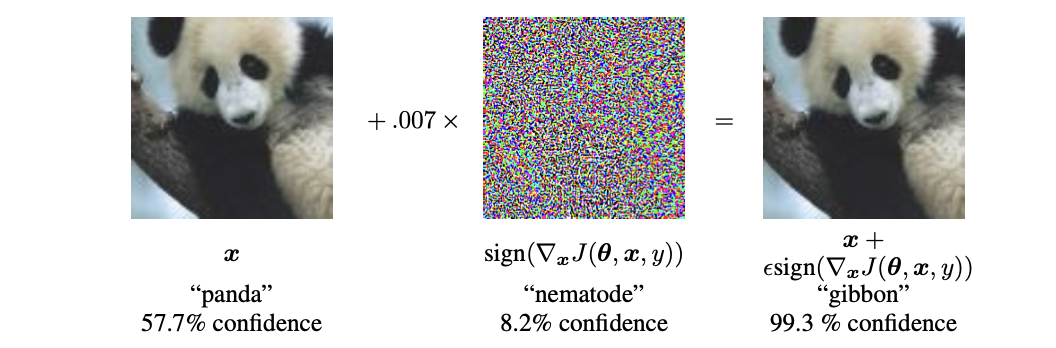
\includegraphics[width=0.8\textwidth]{figures/fgsm.png}
    \caption{Adversarial Example Generated by FGSM}
    \label{fig:panda}
\end{figure}
As discussed , the adversarial space emerges from the imperfect representation of the input space during training. Memorization amplifies this imperfections by increasing the model’s susceptibility to gradient-based perturbations. When a model prioritizes memorizing specific samples over learning generalizable features, the resulting decision boundaries become highly “jagged” and fragile. These boundaries narrow the distance between training data, which attackers can systematically exploit using fast gradient sign method to shift  the input into incorrect classification zone. 
\paragraph{Projected Gradient Descent (PGD)}
While FGSM provides single-step attacks , PGD provides iterative approach by applying small perturbations to the input data to maximize the model’s prediction error. Based on the information given in \cite{aleksander_m_dry_8d27e246}, the inner problem is to find a perturbation that causes the greatest increase in loss function. In prior studies , the linearization approach that is used in FGSM , a single step approach , is not enough to understand the inner problem in more detail. The iterative nature of PGD allows for a more exhaustive search for adversarial examples repeatedly applying first-order gradients to navigate the complex loss landscape. In the experiment provided in \cite{aleksander_m_dry_8d27e246}, states that given datasets of MNSIT and CIFAR-10 , the adjusted PGD attack consistently outperformed FGSM in terms of attack success, with a higher percentage  of loss maximization with CIFAR-10 dataset. Even though MNSIT and CIFAR-10 are robust to adversarial attacks, MNSIT achieves high accuracy for wide range of powerful ℓ∞-bound adversaries and large perturbations due to the large fraction of atypical samples contained in CIFAR-10 .

Furthermore, Memorization amplifies the effectiveness of PGD by exploiting the model’s vulnerabilities in training by generating a very jagged loss landscape. While PGD is a first-order (gradient-based) adversary, if the gradients are “shattered“ or “noisy“ due to memorization, PGD might get stuck in poor local maximum, making the model appear  robust when it actually isn’t.

\clearpage
%%%%%%%%%%%%%%%%%%%%%%%%%%%%%%%%%%%%%


%%%%%%%%%%%%%%%%%%%%%%%%%%%%%%%%%%%%%


























